\chapter{Implementation Issues}
%\addcontentsline{toc}{chapter}{Appendix A: Implementation Issues}

\section{Working with Files}

XMF is a dynamic engine that runs program code loaded from files.
Files can be loaded at any time and the definitions come into immediate
effect. It is usual for the files to be loaded form the top-level
command loop (although loading files from an executing program is
also possible). Files have a '.xmf.' extension and have a specific
format:

\begin{lstlisting}
<PARSER_IMPORT>*

<IMPORT>*

(<DEFINITIONS> | <COMMAND>)*
\end{lstlisting}The parse imports are used to place syntax classes into scope for
the rest of the file. If a syntax class C is in scope then the file
may contain constructs of the form @C ... end. When the XMF parser
encounters such a construct it looks up the syntax classes in scope,
finds a class named C and uses the grammar of C to parse the construct
and to synthesize a performable element. Each parse import has the
form:

\begin{lstlisting}
parserImport <PATH>;
\end{lstlisting}where a path references a name-space containing syntax classes. Typically
a file will contain a single parser-import for the name-space XOCL;
this name-space contains all the syntax classes for XOCL definitions
such as For, Class, Package, attribute etc.

The imports are used to place named elements in scope for the rest
of the file. Each import references a name-space whose named elements
can be referenced within the file without further qualification. Each
import has the form:

\begin{lstlisting}
import <PATH>;
\end{lstlisting}A definition is used to add an element to a container; typically adding
a named element to a name-space. A definition has the form:

\begin{lstlisting}
context <PATH>
  <EXP>
\end{lstlisting}where the path references a name-space and the expression evaluates
to produce a named element. On loading the file the expression is
evaluated, added to the name-space and then initialised (causing any
internal references to be resolved). Typically, definitions are used
to create class and package definitions. 

Definitions are also used to add operations to classes. It is usual
to spread the definition of a package and a class over several files,
each file contains the definition of various related features. For
example a package may be defined in a file, its classes in several
files and then the operations for each class in several further files.
When doing this, care should be taken to load the files in an appropriate
order so that the name-spaces referenced in a definition are available
when the file is loaded.

Commands in files are just XOCL expressions terminated by a ';'. Typically
commands are used for their side-effect.

Here is a typical file:

\begin{lstlisting}
parserImport XOCL;

import MyModels;
import MyPackage;

// Add a new class. Notice that MyClass
// is imported and needs no further
// qualification...

context MyPackage
  @Class NewClass extends MyClass
    @Attribute x : MyClass end
  end

// Extend MyModels::MyPackage::MyClass...

context MyClass
  @Operation myOp()
    // Some Body
  end
\end{lstlisting}A source file is compiled using the operation:

\begin{lstlisting}
Compiler::compileFile(String,Boolean,Boolean)
\end{lstlisting}This operation takes three arguments: the path to the source file
and two boolean values both of which should be true. If the file compiles
correctly then the resulting binary file has an extension '.o' and
can be loaded using String::loadBin(). The top-level command loop
has some useful commands that make it easy to compile and load files.
The paths are supplied without file extensions:

\begin{lstlisting}
?c  <PATH>     // Compile the source file.
?cl <PATH>     // Compile then load the source file.
?l  <PATH>     // Load gthe binary file.
?c             // Compile the last supplied path.
?l             // Load the last supplied path.
\end{lstlisting}
\section{Manifests}

XOCL applications tend to run to a number of files. It is possible
to write a single file containing directives to compile and load the
application files in the correct order, however this becomes difficult
to manage since paths have to be absolute etc. The manifest language
construct works like a make-file: it is used to list all the files
in a module and all the sub-modules. The manifest uses paths relative
to a root so that the module is easily relocatable. In addition manifests
include some useful directives that can be used to control the compilation
and loading of the module.

A manifest file is called Manifest.xmf and has the following structure:

\begin{lstlisting}
parserImport Manifests;

@Manifest <NAME>
  <DIRECTIVE>*
end;
\end{lstlisting}The name of the manifest is just used for documentation. A manifest
file occurs in a directory, all directives in the manifest are relative
to this directory. A directive refers either to a file or a directory.
A file directive has the following form:

\begin{lstlisting}
@File [^<LOADTIME>] <PATH> end
\end{lstlisting}The optional load-time directive specifies when the file should be
loaded. A manifest is used to both compile and load files; load-time
directives are one of:

CompileTime; RunTime; Both; None. The path to the file is relative
to the directory containing the manifest and should be specified with
no file extension. Whe the manifest is used to compile entries, a
file is compiled if the source (.xmf) is out of date with respect
to the binary (.o). Once compiled if the load-time directive is specified
as CompileTime or Both then the file is loaded. When the manifest
is used to load entries, the binary is loaded providing that the load-time
directive is not specified or is RunTime or Both.

A directory directive has the following form:

\begin{lstlisting}
@Ref [^<LOADTIME>] <PATH> end
\end{lstlisting}where the path references a sub-directory that contains a manifest
file. On compilation, the referenced manifest is loaded and its entries
compiled. On loading, the referenced manifest is loaded and its entries
are loaded.

The following is a typical manifest:

\begin{lstlisting}
parserImport Manifests;

@Manifest MyModule
  @File MyPackage end
  @File MyTopLevelClass end
  @File SomeOperations end
  @Ref MyFirstSubPackage end
  @Ref MySecondSubPackage end
end;
\end{lstlisting}Manifests can be used under program control:

\begin{lstlisting}
// Load the manifest file...
let m = "someDir/Manifest.o".loadBin()
in // Use the manifest to compile the entries.
   // Supply the directory containing the 
   // manifest...
   m.build("someDir");
   // Use the manifest to load the entries...
   m.load("someDir")
end
\end{lstlisting}The top-level command loop provides commands that make it easy to
use manifests. In the following, <PATH> refers to a directory containing
a manifest file:

\begin{lstlisting}
?m b  <PATH>   // Compile entries.
?m l  <PATH>   // Load entries.
?m d  <PATH>   // Delete binaries.
?m bl <PATH>   // Build then load entries.
\end{lstlisting}
\section{XMF Startup Arguments}

XMF can be started from a batch file or from Java. In both cases initialisation
arguments are supplied to the VM as it starts up. These arguments
are detailed below. Subsequent sections describe how these arguments
are supplied to the different ways of starting XMF.

\begin{itemize}
\item -arg {\tt <NAME>:<VALUE>} The global object named xmf contains a collection
of name/value pairs that are supplied via this initialzation argument
designator. The name and the value are separated using :. The collection
of supplied arguments can be referenced as xmf.startupArgs(). Given
a name n for an argument, the value is found as {\tt xmf.startupArgs()->lookup(n)}.
\item -filename {\tt <FILE>}. Specifies a binary file containing a replacement
for the XMF top-level command loop when running the evaluator image
(see below). When starting the evaluator image, if this argument designator
is supplied then the contents are loaded and executed instead of starting
the command loop. When the file completes then the XMF VM terminates.
\item -heapSize {\tt <SIZE>}. The size of the XMF heap is set using this initialisation
argument designator. The size should be a value in XMF VM words and
must be sufficiently large to accommodate any specified image bearing
in mind that the Java VM will manage two heaps (for garbage collection)
of the specified size. A standard size is 10000.
\item -initfile {\tt <FILE>}. When the eval.img image starts (see below) it will,
by default, start a top-level command loop. Before the loop starts
the supplied binary file is loaded.
\item -image {\tt <FILE>}. When the XMF VM starts it loads a saved XMF image into
the heap and continues to run the image from the point at which the
image was saved. This argument designator specified the file containing
the image. For the standard command-line XMF engine, use Images/eval.img.
\item -port {\tt <INT>}. Specifies a port that is used by the XMV VM for socket
connections.
\item -stackSize {\tt <SIZE>}. Specifies the size of the XMF VM stack in machine
words. XMF implements tail calling, so it is not usually necessary
to specify this argument designator.
\end{itemize}
A minimal startup is:

\begin{lstlisting}
-image %XMFHOME%\Images\eval.img -heapSize 10000
\end{lstlisting}
\section{Starting XMF using a Batch File}

There is an example startup file bin/xos.bat for starting the XMF
VM with the top-level command loop defined in eval.img. Run this supplying
the value of XMFHOME to start a top-level command loop:

\begin{lstlisting}
%XMFHOME%\bin\xos %XMFHOME%
\end{lstlisting}or by supplying a filename to replace the top-level loop:

\begin{lstlisting}
%XMFHOME%\bin\xos %XMFHOME% -filename <FILE>
\end{lstlisting}
\section{Starting XMF from Java}

The XMF VM can be started from Java as follows:

\begin{lstlisting}
String[] args = {"-heapSize","10000","-image",XMFHOME + "/Images/eval.img"};
XOS.OperatingSystem os = new XOS.OperatingSystem();
os.init(args)
\end{lstlisting}Different combinations of arguments can be supplied as required.


\section{Rebuilding XMF}

Rebuilding XMF is in two stages (for mainly historical reasons). Assuming
you have all the binaries recompiled (see the next section):

\begin{lstlisting}
%XMFHOME%\bin\makexmf %XMFHOME%
\end{lstlisting}The above creates a new image in XMFHOME\textbackslash{}Images\textbackslash{}xmf.img.
This is a basic image that supports XOCL etc. The next step extends
this image by loading libraries most of which are essential to run
the top-level command loop:

\begin{lstlisting}
%XMFHOME%\bin\makexmf %XMFHOME%
\end{lstlisting}A fresh XMFHOME\textbackslash{}Images\textbackslash{}eval.img is created.


\section{Recompiling XMF}

XMF can be recompiled only from a valid XMF top-level command loop
which requires a valid eval.img. This is done as follows:

\begin{lstlisting}
C:\xmf>bin\xos .
[ bin/xos .         ]
[ Starting XOS ]
[ Load ./Images/eval.img ]

XMF Copyright (C) Xactium Ltd, 2003-2007.

Version 1.9

Type ?h for top level help.

[1] XMF> ?m b .
[ Loading ./Manifest.o...................... 0:0:0:109 ms ]
[ Loading ./Kernel/Manifest.o............... 0:0:0:125 ms ]
[ ./Kernel/Boot.o......................... is up to date. ]
[ ./Kernel/Kernel.o....................... is up to date. ]
[ ./Kernel/Doc.o.......................... is up to date. ]
[ ./Kernel/Attribute.o.................... is up to date. ]
[ ./Kernel/Bind.o......................... is up to date. ]
[ ./Kernel/Boolean.o...................... is up to date. ]
[ ./Kernel/Boot.o......................... is up to date. ]
[ ./Kernel/Buffer.o....................... is up to date. ]
[ ./Kernel/Class.o........................ is up to date. ]
[ ./Kernel/Classifier.o................... is up to date. ]
// Lots more compilation printout....
\end{lstlisting}If you modify the XMF sources in any way then you will need to recompile
and the rebuild to create a fresh image. The rebuilsing process is
describes in the previous section.


\section{Debugging}

Operations can be traced so that information is printed out when the
operation is entered and when it is exited. The output is intended
to reflect the call nesting. Use Operation::trace() to set tracing
and Operation::untrace() to remove tracing. Use Container::traceAll()
to trace all operations in a name-space and Container::untraceAll()
to remove all tracing.


\section{Boolean Operations}

The following list shows the main operations defined by the datatype
Boolean:

\begin{lstlisting}
Boolean::booland(other:Boolean):Boolean
Boolean::boolor(other:Boolean):Boolean
Boolean::boolnot():Boolean
\end{lstlisting}
\section{Float Operations}

The following list shows the main operations defined by the datatype
Float:

\begin{lstlisting}
Float::abs():Integer
Float::add(other::Float):Float
Float::ceiling():Integer
Float::cos():Float
Float::floor():Integer
Float::random():Float
Float::sun():Float
Float::slash(other:Float):Float
\end{lstlisting}
\section{Integer Operations}

The following list shows the main operations defined by the datatype
Integer:

\begin{lstlisting}
Integer::add(other:Integer):Integer
Integer::bit(offset:Integer):Integer
Integer::byte(offset:Integer):Integer
Integer::div(other:Integer):Integer
Integer::greater(other:Integer):Integer
Integer::isAlphaChar():Boolean
Integer::isLowerCaseChar():Boolean
Integer::isnewLineChar():Boolean
Integer::isNumericChar():Boolean
Integer::isUpperCaseChar():Boolean
Integer::isWhiteSpaceChar():Boolean
Integer::less(other:Integer):Boolean
Integer::lsh(offset):Integer
Integer::max(other:Integer):Integer
Integer::min(other:Integer):Integer
Integer::mod(other:Integer):Integer
Integer::mul(other:Integer):Integer
Integer::pow(power:Integer):Integer
Integer::random(upper:Integer):Integer
Integer::rsh(offset:Integer):Integer
Integer::slash(Integer):Float
Integer::sqrt():Float
Integer::sub(other:Integer):Integer
Integer::to(upper:Integer):Seq(Integer)
\end{lstlisting}
\section{Sequence Operations}

The following list shows the main operations defined by the datatype
Seq(Element):

\begin{lstlisting}
Seq(Element)::append(other:Seq(Element)):Seq(Element)
Seq(Element)::asSeq():Seq(Element)
Seq(Element)::asSet()::Set(Element)
Seq(Element)::asString():String
Seq(Element)::asVector():Vector
Seq(Element)::assoc(key):Seq(Element)
Seq(Element)::at(i:Integer)
Seq(Element)::bind(key,value):Seq(Element)
Seq(Element)::butLast():Seq(Element)
Seq(Element)::collect(pred:Operation):Seq(Element)
Seq(Element)::contains(element):Boolean
Seq(Element)::delete(element):Seq(Element)
Seq(Element)::drop(n:Integer):Seq(Element)
Seq(Element)::excluding(element):Seq(Element)
Seq(Element)::exists(pred:Operation):Boolean
Seq(Element)::flatten():Seq(Element)
Seq(Element)::forAll(pred:Operation):Boolean
Seq(Element)::hasPrefix(p:Seq(Element)):Boolean
Seq(Element)::head()
Seq(Element)::includes(Element):Boolean
Seq(Element)::includesAll(other:Seq(Element):Boolean
Seq(Element)::including(element):Seq(Element)
Seq(Element)::indexOf(element):Integer
Seq(Element)::insertAt(element,index:Integer):Seq(Element)
Seq(Element)::intersection(other:Seq(Element)):Seq(Element)
Seq(Element)::isEmpty():Boolean
Seq(Element)::isProperSequence():Boolean
Seq(Element)::iter(iter:Operation,start)
Seq(Element)::last()
Seq(Element)::lookup(key)
Seq(Element)::map(name:String):Seq(Element)
Seq(Element)::max():Integer
Seq(Element)::mul(other:Seq(Element)):Seq(Element)
Seq(Element)::prepend(element):Seq(Element)
Seq(Element)::qsort():Seq(Element)
Seq(Element)::sortNamedElements:Seq(Element)
Seq(Element)::subSequence()
Seq(Element)::subst(new,old,all):Seq(Element)
Seq(Element)::tail()
Seq(Element)::take(n:Integer):Seq(Element)
Seq(Element)::unbind(key):Seq(Element)
Seq(Element)::zip(other:Seq(Element)):Seq(Element)
\end{lstlisting}
\section{Set Operations}

The following list shows themain operations defined by the datatype
Set(Element):

\begin{lstlisting}
Set(Element)::asSeq():Seq(Element)
Set(Element)::asSet()::Set(Element)
Set(Element)::collect(pred:Operation):Set(Element)
Set(Element)::contains(element):Boolean
Set(Element)::excluding(element):Set(Element)
Set(Element)::exists(pred:Operation):Boolean
Set(Element)::flatten():Set(Element)
Set(Element)::forAll(pred:Operation):Boolean
Set(Element)::includes(Element):Boolean
Set(Element)::includesAll(other:Set(Element):Boolean
Set(Element)::including(element):Set(Element)
Set(Element)::intersection(other:Set(Element)):Set(Element)
Set(Element)::isEmpty():Boolean
Set(Element)::iter(iter:Operation,start)
Set(Element)::map(name:String):Set(Element)
Set(Element)::max():Integer
Set(Element)::mul(other:Set(Element)):Set(Element)
Set(Element)::power():Set(Element)
Set(Element)::sel()
Set(Element)::size():Integer
Set(Element)::union(other::Set(Element)):Set(Element)
\end{lstlisting}
\section{String Operations}

The following list shows the main operations defined by the datatype
String:

\begin{lstlisting}
String::asBool():Boolean
String::asFloat():Float
String::asInt():Integer
String::asSeq():Seq(Integer)
String::asXML():XML::Element
String::at(i:Integer):Integer
String::fileExists():Boolean
String::greater(other:String):Boolean
String::hasPrefix(p:String):Boolean
String::hasSuffix(s:String):Boolean
String::isDir():Boolean
String::loadBin()
String::lowerCase():String
String::lowerCaseInitialLetter():String
String::mkDir():Boolean
String::size():Integer
String::splitBy(chars:String,start:Integer,last:Integer):Seq(String)
String::subst(new:String,old:String,all:Boolean):String
String::toLower():String
String::toUpper():String
\end{lstlisting}

\section{OCL Syntax Classes\label{sec:OCL-Syntax-Classes}}

This section defines the classes that make up the Object Command Language
(the core part of XOCL). They are defined in the package OCL. The
syntax classes are grouped roughly in terms of their basic properties
and usage.

%
\begin{figure}
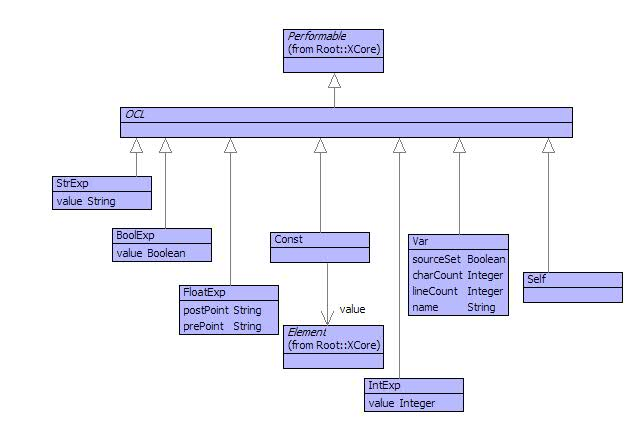
\includegraphics[scale=0.6]{Appendix/Images/Atomic}
\caption{Atomic Expressions\label{fig:Atomic-Expressions}}
\end{figure}


%
\begin{figure}
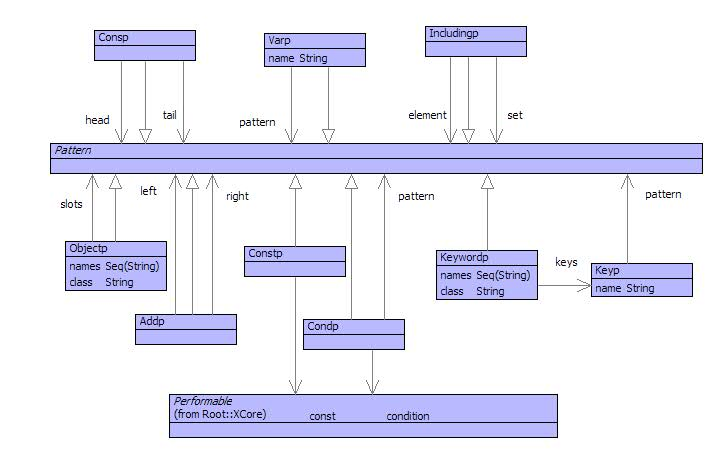
\includegraphics[scale=0.75,angle=90]{Appendix/Images/Pattern}
\caption{Pattern Expressions\label{fig:Pattern-Expressions}}
\end{figure}


Figure \ref{fig:Atomic-Expressions} shows classes for atomic expressions.
Figure \ref{fig:Pattern-Expressions} shows the classes for patterns
that occur in argument positions of operation expressions (and in
@Case expressions). Briefly, Consp is a pair pattern, Varp is a simple
variable, Includingp is a set pattern, Objectp is a pattern corresponding
to a constructor, Addp is a sequence concatenation or set union pattern,
Constp is a constant (where the constant is the result of evaluating
an expression), Condp is a guard and Keywordp is a pattern matching
objects where the slots are given as keys.

%
\begin{figure}
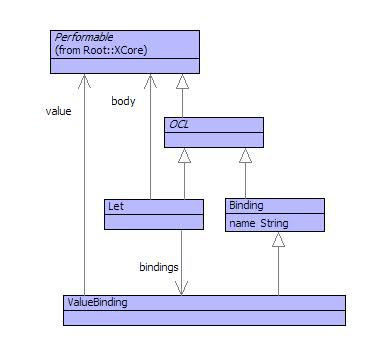
\includegraphics[scale=0.75]{Appendix/Images/Let}
\caption{Let Expressions\label{fig:Let-Expressions}}
\end{figure}


%
\begin{figure}
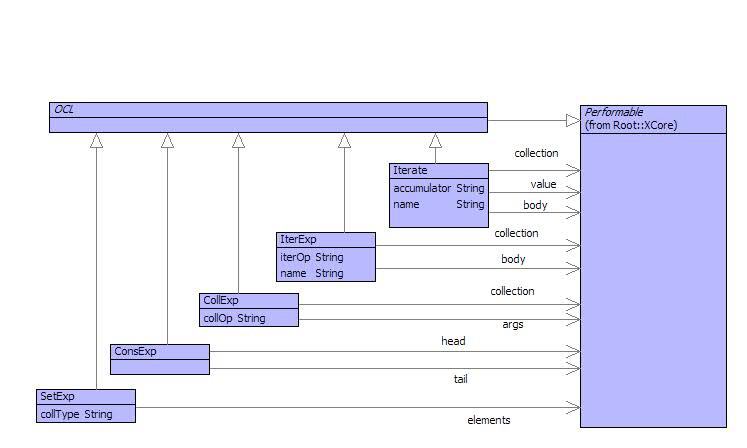
\includegraphics[scale=0.75,angle=90]{Appendix/Images/Iteration}
\caption{Iteration Expressions\label{fig:Iteration-Expressions}}
\end{figure}


Figure \ref{fig:Let-Expressions} shows the syntax of let-expressions.
Figure \ref{fig:Iteration-Expressions} shows the classes for iteration
expressions. Both set and sequence expressions are represented as
instances of SetExp with the collType set to Set or Seq respectively.
A CollExp supports all concrete expressions of the form {\tt S->x(a,b,c)}
and {\tt S->x} where the arguments to the latter default to the empty sequence.
IterExp represents all concrete expressions of the form {\tt S->n(x | e)}
where n is exists, forAll, select, collect or reject.

%
\begin{figure}
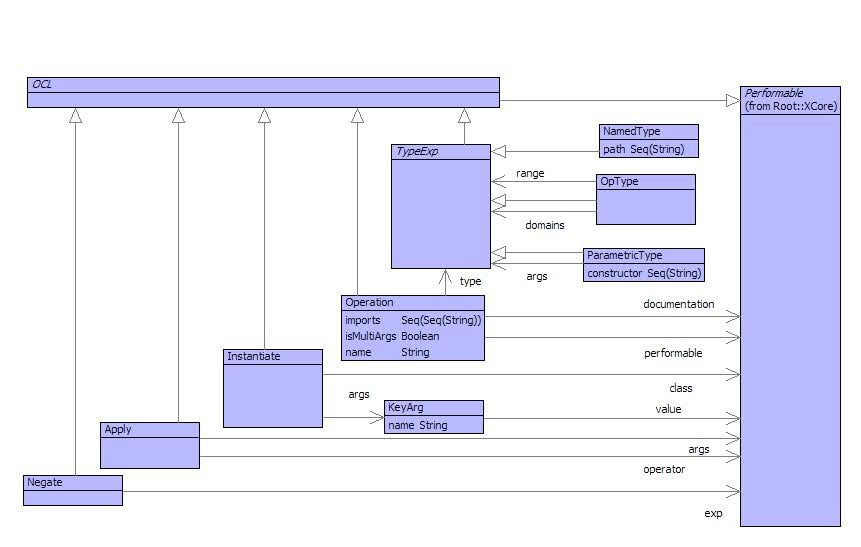
\includegraphics[scale=0.75,angle=90]{Appendix/Images/Ops}
\caption{Operation Expressions\label{fig:Operation-Expressions}}
\end{figure}


%
\begin{figure}
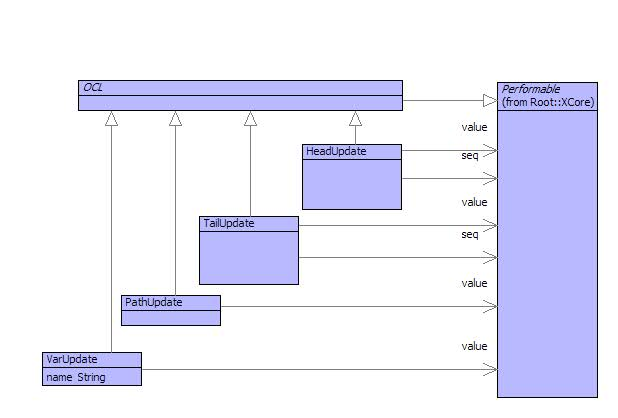
\includegraphics[scale=0.75,angle=90]{Appendix/Images/Update}
\caption{Update Expressions\label{fig:Update-Expressions}}
\end{figure}


Figure \ref{fig:Operation-Expressions} shows the classes for operations.
Note that operation arguments are not shown but are an attribute of
type Seq(Pattern). Figure\ref{fig:Update-Expressions} shows the classes
for update expressions. Updates can be variable, x := e, path P::Q::x
:= e, or head and tail: {\tt s->head := e} and {\tt s->tail := e}. 

%
\begin{figure}
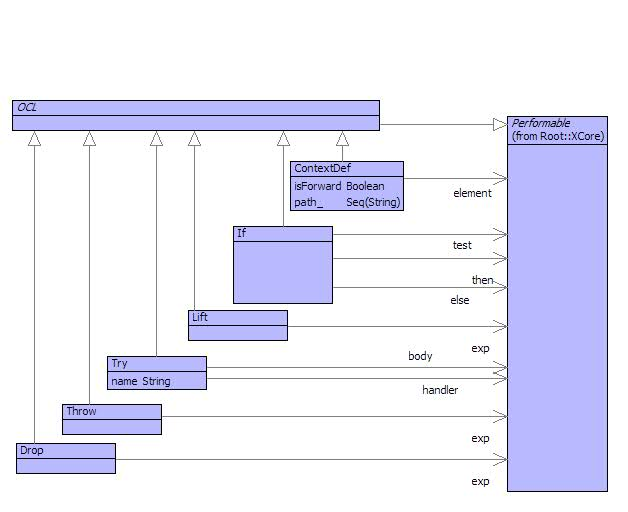
\includegraphics[scale=0.75,angle=90]{Appendix/Images/Misc}
\caption{Misc Expressions\label{fig:Misc-Expressions}}
\end{figure}


Figure \ref{fig:Misc-Expressions} shows the rest of the expression
types.
